\documentclass[assignment02_Solutions]{subfiles}

%\IfSubStr{\jobname}{\detokenize{Solutions}}{\toggletrue{solutions}}{\toggletrue{solutions}}
\IfSubStr{\jobname}{\detokenize{Solutions}}{\toggletrue{solutions}}{\togglefalse{solutions}}

\invalidatemargin

\fancypagestyle{firstpage}

{\rhead{Assignment 2 \linebreak \textit{Version: \today}}}

\title{Assignment 2: Classification and Linear Regression}
\author{Machine Learning}
\date{Fall 2021}

\begin{document}

\maketitle
\thispagestyle{firstpage}



\begin{learningobjectives}
\bi
\item Implement a simple classification algorithm in Python
\item Learn mathematical tricks for manipulating matrices and vectors.
\item Derive the linear regression algorithm
\item Implement linear regression in Python
\ei
\end{learningobjectives}

\begin{priorknowledge}
\bi
\item Supervised learning problem framing
\item Setup for the linear regression problem
\item Partial derivatives and gradients, matrix-vector multiplication, and vector-vector multiplication
\ei
\end{priorknowledge}

\section{Supervised Learning Framing}

In the last assignment, you saw a high level overview of machine learning broken into the categories of supervised, unsupervised, and reinforcement learning (see figure below). Supervised learning can be split into regression (predicting a quantity) and classification (predicting a label). In this assignment, we will look at an example of classification, and then dig deeper into linear regression. 

\begin{figure}
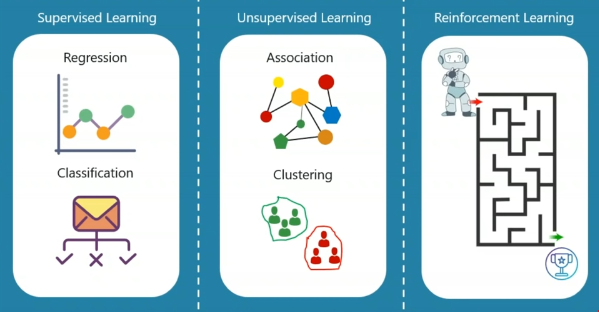
\includegraphics[width=0.7\linewidth]{figures/SupervisedUnsupervisedReinforcement}
\centering
%\caption{Image from \href{https://medium.com/analytics-vidhya/introduction-to-machine-learning-regression-5bbf4ed96f40}{Esma Bozkurt}}% https://medium.com/analytics-vidhya/introduction-to-machine-learning-regression-5bbf4ed96f40}
\centering
\end{figure}
\begin{center}
Image from Esma Bozkurt \href{https://medium.com/analytics-vidhya/introduction-to-machine-learning-regression-5bbf4ed96f40}{article on medium.com}
\end{center}


	

\section{Implement classification with a train/test split}

As we (hopefully) learned in the class activity, overfitting our model to our data can lead to diminished results when we apply our model to a new set of data. One of the ways we try to avoid overfitting is by splitting our data into a training and testing set. (In the future, we will talk about another split of the training data called cross-validation, but for now, we won't worry about that.)


\begin{externalresources}[(60 minutes)]
Work through the \href{https://colab.research.google.com/drive/1d4EvlaSpgGB-hx78Kj2ii5ee7dczW-I5?usp=sharing}{Assignment 2a Companion Notebook} to practice implementing a simple classification algorithm called a decision tree in Python. You can place your answers directly in the Jupyter notebook so that you have them for your records.
\end{externalresources}



\section{A Quick Refresher on Linear Regression}

In the last assignment you worked with the linear regression (ordinary least-squares) algorithm from a top-down perspective.  We focused on what problem the algorithm is trying to solve (minimizing squared error) and then showed some of the algorithm's behavior when applied to a toy problem.

In this part of the assignment we are going to focus on linear regression from the bottom up.  We will be working through the mathematics (and eventually the implementation in code) of the solution to the linear regression problem.  Before diving in, we thought it would be helpful to include some reminders of the setup for the generic supervised learning problem and the setup for linear regression.  If you already feel good about these topics, you can safely skip to the next section.

\vspace{1em}

\begin{recall}[Supervised Learning Problem Setup]
We are given a training set of data instances, $(\mlvec{x_1}, y_1), (\mlvec{x}_2, y_2), \ldots, (\mlvec{x}_n, y_n)$ where each $\mlvec{x_i}$ represents an element of an input space (e.g., a d-dimensional feature vector) and each $y_i$ represents an element of an output space (e.g., a scalar target value).  Our goal is to determine a function $\hat{f}$ that maps from the input space to the output space.

We assume there is a loss function, $\ell$, that determines the amount of loss that a particular prediction $\hat{y}_i$ incurs due to a mismatch with the actual output $y_i$.  The best possible model, $\hat{f}^\star$, is the one that minimizes these losses over the training set.  This notion can be expressed with the following equation.
\begin{align}
\hat{f}^\star &= \argmin_{\hat{f}} \sum_{i=1}^n \ell \left ( \hat{f}(\mlvec{x_i}), y_i \right )
\end{align} 

\end{recall}

\vspace{1em}


\begin{recall}[The Linear Regression Model]

Our input points, $\mlvec{x_i}$, are d-dimensional vectors (each entry of these vectors can be thought of as a feature), our output points, $y_i$, are scalars, and our prediction functions, $\hat{f}$, are all of the form $\hat{f}(\mlvec{x}) = \mlvec{w}^\top \mlvec{x} = \sum_{i=1}^d w_i x_i$ for some weights $\mlvec{w}$.

In the function, $\hat{f}$, the elements of the vector $\mlvec{w}$ represent weights that multiply various entries of the input.  For instance, if an element of $\mlvec{w}$ is high, that means that as the corresponding element of $\mlvec{x}$ increases, the prediction that $\hat{f}$ generates for $\mlvec{x}$ would also increase.  The products of the weights and the features are then summed to arrive at an overall prediction.

Given this model, we can now define the \href{https://en.wikipedia.org/wiki/Ordinary_least_squares}{ordinary least squares} (OLS) algorithm!  In the ordinary least squares algorithm, we use our training set to select the $\mlvec{w}$ that minimizes the sum of squared differences between the model's predictions and the training outputs.  This corresponds to choosing $\ell(y, \hat{y}) = (y - \hat{y})^2$.

\begin{align}
\mlvec{w}^\star &= \argmin_{\mlvec{w}} \sum_{i=1}^n \ell \left ( \hat{f}(\mlvec{x_i}, \mlvec{w}) , y_i \right) \\
&= \argmin_{\mlvec{w}} \sum_{i=1}^n \left ( \hat{f}(\mlvec{x_i}, \mlvec{w}) - y_i \right)^2 \\
&= \argmin_{\mlvec{w}} \sum_{i=1}^n \left ( \mlvec{w}^\top \mlvec{x_i} - y_i \right)^2
\end{align}

Once we have $\mlvec{w}^\star$, we can predict the unknown output, $y$, for a new input point, $\mlvec{x}$, as $\hat{y} = \mlvec{w^\star}^\top \mlvec{x}$.
\end{recall}

\section{Linear Regression from the Bottom-up}

Now that we've refreshed ourselves on the basic framing of linear regression, we'll be diving into the mathematics of how to find the vector $\mlvec{w}^\star$ that best fits a particular training set.  The outline of the steps we are going to take to learn this are:

\be
\item Solve the special case of linear regression with a single input ($d=1$, meaning a 1-dimensional feature vector).
\item Learn some mathematical tricks for manipulating matrices and vectors and computing gradients of functions involving matrices and vectors (these will be useful for solving the general case of linear regression).
\item Solve the general case of linear regression (where $d$ can be any positive, integer value).
\ee

\subsection{Linear regression with one variable}

\begin{exercise}[(20 minutes)]
\bes
\item Given a dataset $(x_1, y_1), (x_2, y_2), \ldots, (x_n, y_n)$ (where each $x_i$ and each $y_i$ is a scalar) and a potential value of $w$ (note that $w$ is a scalar in the case where $d=1$), write an expression for the sum of squared errors between the model predictions, $\hat{f}$, and the targets, $y_i$.  \textbf{Note:} In contrast to the line of best fit we saw in the last assignment, here we are not computing a y-intercept (effectively forcing the y-intercept to be $0$).  This choice may result in a worse fit, but it is easier to work out and helps build mathematical intuition.

\begin{boxedsolution}
\begin{align}
\mbox{Sum of Squared Errors} &= e(w) = \sum_{i=1}^n \left (  w x_i - y_i \right)^2~~\mbox{(note: we define error $e(w)$ for convenience)}
\end{align}
\end{boxedsolution}

\item Compute the derivative of the expression for the sum of squared errors from part (a).

\begin{boxedsolution}
\begin{align}
\frac{de}{dw} & = \sum_{i=1}^n 2 \left (  w x_i - y_i \right)x_i  \\
&= w \sum_{i=1}^n 2 x_i^2 - \sum_{i=1}^n 2 x_i y_i
\end{align}
\end{boxedsolution}

\item Set the derivative to 0, and solve for $w^\star$.  $w^\star$ corresponds to a critical point of your sum of squared errors function.  Is this critical point a minimum, maximum, or neither? (here is a refresher on \href{http://homes.sice.indiana.edu/donbyrd/Teach/M119WebPage/Finding+ClassifyingCriticalPoints.pdf}{classifying critical points}).
 
\begin{boxedsolution}
\begin{align}
\frac{de}{dw} &= 0 \\
&= w^\star \sum_{i=1}^n 2 x_i^2 - \sum_{i=1}^n 2 x_i y_i \\
\sum_{i=1}^n 2 x_i y_i  &= w^\star \sum_{i=1}^n 2 x_i^2 \\
w^\star &=\frac{\sum_{i=1}^n x_i y_i}{\sum_{i=1}^n x_i^2}
\end{align}

If we take the second derivative of $e(w)$ we get:
\begin{align}
\frac{d^2e}{dw^2} &= \sum_{i=1}^n 2x_i^2 \enspace .
\end{align}

We can see from the form of the second derivative that it is always non-negative, and therefore the critical point at $w^\star$ corresponds to a minimum.
\end{boxedsolution}
\ees


\end{exercise}

\subsection{Reminder of mathematical ideas from the last assignment}

In the previous assignment, we asked you to solidify your knowledge of three different mathematical concepts.  The box below summarizes what you were supposed to learn and provides the resources we provided to help you.

\vspace{1em}
\begin{recall}[Mathematical background]
In order to engage with this assignment, you'll want to make sure you are familiar with the following concepts (links to resources embedded below):
\bi
\item vector-vector multiplication
\bi
\item Section 2.1 of \href{https://see.stanford.edu/materials/aimlcs229/cs229-linalg.pdf}{Zico Kolter's Linear Algebra Review and Reference}
\ei
\item Matrix-vector multiplication
\bi
\item Section 2.2 of \href{https://see.stanford.edu/materials/aimlcs229/cs229-linalg.pdf}{Zico Kolter's Linear Algebra Review and Reference}
\item The first bits of the Khan academy video on \href{https://www.khanacademy.org/math/linear-algebra/matrix-transformations/linear-transformations/v/matrix-vector-products-as-linear-transformations}{Linear Transformations}
\ei
\item partial derivatives and gradients
\bi
\item Khan Academy videos on partial derivatives: \href{https://www.khanacademy.org/math/multivariable-calculus/multivariable-derivatives/partial-derivatives/v/partial-derivatives-introduction}{intro}, \href{https://www.khanacademy.org/math/multivariable-calculus/multivariable-derivatives/partial-derivatives/v/partial-derivatives-and-graphs}{graphical understanding}, and \href{https://www.khanacademy.org/math/multivariable-calculus/multivariable-derivatives/partial-derivatives/v/formal-definition-of-partial-derivatives}{formal definition}
\item \href{https://www.khanacademy.org/math/multivariable-calculus/multivariable-derivatives/gradient-and-directional-derivatives/v/gradient}{Khan Academy video on Gradient}
\ei
\ei
\end{recall}


\subsection{Building our bag of mathematical tricks}

The derivation of linear regression for the single variable case made use of your background from single variable calculus, and you used some rules for manipulating such functions.  When approaching linear regression with multiple variables, you have two choices.
\be
\item You can apply the same bag of tricks you used for the single variable problem and only at the end convert things (necessarily) to a multivariable representation.  
\item You can approach the whole problem from a multivariable perspective.
\ee

This second approach requires that you learn some additional mathematical tricks, but once you learn these tricks, the derivation of linear regression is very straightforward.  The secondary benefit of this approach is that the new mathematical tricks you learn will apply to all sorts of other problems.

\begin{exercise}[(15 minutes)]
A quadratic form can be expressed in matrix-vector form as $\mlvec{x}^\top \mlmat{A} \mlvec{x}$.  Written this way, it looks very mysterious, but in this exercise you'll build some intuition about what the expression represents. Further, it turns out that expressions like this show up in all sorts of places in machine learning.   To get a better understanding of what a quadratic form \emph{is} (we'll see what it's good for later), watch this \href{https://www.khanacademy.org/math/multivariable-calculus/applications-of-multivariable-derivatives/quadratic-approximations/v/expressing-a-quadratic-form-with-a-matrix}{Khan Academy video}.

After you've watched the Khan academy video, answer these questions.

\bes
\item Multiply out the expression $\begin{bmatrix} x_1 \\ x_2 \\ x_3 \end{bmatrix}^\top \begin{bmatrix} a_{1,1} & a_{1,2} & a_{1,3} \\ a_{2,1} & a_{2,2} & a_{2,3} \\ a_{3,1} & a_{3,2} & a_{3,3} \end{bmatrix}\begin{bmatrix} x_1 \\ x_2 \\ x_3 \end{bmatrix}$.

\begin{boxedsolution}
\begin{align}
\begin{bmatrix} x_1 \\ x_2 \\ x_3 \end{bmatrix}^\top \begin{bmatrix} a_{1,1} & a_{1,2} & a_{1,3} \\ a_{2,1} & a_{2,2} & a_{2,3} \\ a_{3,1} & a_{3,2} & a_{3,3} \end{bmatrix}\begin{bmatrix} x_1 \\ x_2 \\ x_3 \end{bmatrix} =&  \begin{bmatrix} x_1 \\ x_2 \\ x_3 \end{bmatrix}^\top \begin{bmatrix} a_{1,1} x_1 + a_{1,2} x_2 + a_{1,3} x_3 \\ a_{2,1} x_1 + a_{2,2} x_2 + a_{2,3} x_3 \\ a_{3,1} x_1 + a_{3,2} x_2 + a_{3,3} x_3 \end{bmatrix} \\
=& a_{1,1} x_1^2 + a_{1,2}x_1x_2 + a_{1,3} x_1 x_3 + a_{2,1}x_1 x_2 + a_{2,2} x_2^2  \nonumber \\
&+ a_{2,3} x_2 x_3 + a_{3,1} x_3 x_1 + a_{3,2} x_3 x_2 + a_{3,3} x_3^2
\end{align}
\end{boxedsolution}

\item Complete the following expression by filling in the part on the righthand side inside the nested summation.

$\begin{bmatrix} x_1 \\ x_2 \\ \vdots \\ x_d \end{bmatrix}^\top \begin{bmatrix} a_{1,1} & a_{1,2} & \ldots & a_{1,d} \\ a_{2,1} & a_{2,2} & \ldots & a_{2,d} \\ \vdots & \vdots & \ddots & \vdots \\ a_{d,1} & a_{d,2} & \ldots & a_{d,d} \end{bmatrix}\begin{bmatrix} x_1 \\ x_2 \\ \vdots \\ x_d \end{bmatrix} = \sum_{i=1}^d \sum_{j=1}^d \left (\mbox{your answer here} \right )$

Spoiler alert: Exercise 4 provides you with this result (or, as always, you can check the solutions).

\begin{boxedsolution}
\begin{align}
\begin{bmatrix} x_1 \\ x_2 \\ \vdots \\ x_d \end{bmatrix}^\top \begin{bmatrix} a_{1,1} & a_{1,2} & \ldots & a_{1,d} \\ a_{2,1} & a_{2,2} & \ldots & a_{2,d} \\ \vdots & \vdots & \ddots & \vdots \\ a_{d,1} & a_{d,2} & \ldots & a_{d,d} \end{bmatrix}\begin{bmatrix} x_1 \\ x_2 \\ \vdots \\ x_d \end{bmatrix} &= \begin{bmatrix} x_1 \\ x_2 \\ \vdots \\ x_d \end{bmatrix}^\top \begin{bmatrix} \sum_{j=1}^d a_{1,j} x_j \\ \sum_{j=1}^d a_{2,j} x_j  \\ \vdots \\ \sum_{j=1}^d a_{d,j} x_j \end{bmatrix}\\
&= \sum_{i=1}^d \sum_{j=1}^d a_{i,j}  x_i x_j
\end{align}
\end{boxedsolution}

\ees

\end{exercise}

\begin{exercise}[(5 minutes)]
Matrix multiplication distributes over addition.  That is, $(\mlmat{A} + \mlmat{B}) (\mlmat{C} + \mlmat{D}) = \mlmat{A}\mlmat{C} + \mlmat{A}\mlmat{D} + \mlmat{B} \mlmat{C} + \mlmat{B} \mlmat{D}$.  Use this fact coupled with the fact that $\left(\mlmat{A} \mlmat{B} \right)^\top = \mlmat{B}^\top \mlmat{A}^\top$ to expand out the following expression.

$$\left ( \mlmat{A} \mlmat{x}  + \mlmat{y} \right )^\top \left (\mlmat{v} + \mlmat{u} \right)$$

\begin{boxedsolution}
$$\left ( \mlmat{A} \mlmat{x}  + \mlmat{y} \right )^\top \left (\mlmat{v} + \mlmat{u} \right) = \mlmat{x}^\top \mlmat{A}^\top \mlmat{v} + \mlmat{x}^\top \mlmat{A}^\top \mlmat{u} + \mlvec{y}^\top \mlvec{v} + \mlvec{y}^\top \mlvec{u}$$
\end{boxedsolution}

\end{exercise}

\begin{exercise}[(25 minutes)]
\bes
\item Using the definition of the gradient, show that $\nabla \mlvec{c}^\top \mlvec{x} = \mlvec{c}$ where the gradient is taken with respect to $\mlvec{x}$ and $\mlvec{c}$ is a vector of constants.

\begin{boxedsolution}

\begin{align}
\mlvec{c}^\top \mlvec{x} &= \sum_{j=1}^d c_j x_j \\
\frac{\partial}{\partial x_i}  \sum_{j=1}^d c_j x_j  &= c_i  \\
\nabla \mlvec{c}^\top \mlvec{x} &= \mlvec{c}
\end{align}

\end{boxedsolution}


\item Using the definition of the gradient, show that the $\nabla \mlvec{x}^\top \mlmat{A} \mlvec{x} = 2 \mlmat{A} \mlvec{x}$ where the gradient is taken with respect to $\mlvec{x}$ and $\mlmat{A}$ is a \emph{symmetric} $dxd$ matrix of constants.  Hint: utilize the fact that $\mlvec{x}^\top \mlmat{A} \mlvec{x} = \sum_{i=1}^d\sum_{j=1}^d x_i x_j a_{i, j}$.%  \todo{this might be too hard... Can we make this optional with appropriate sign-posting.... you can prove this is true, but you do not need to do so in order to make progress.  It can also be made easier if you assume $A$ is symmetric.}
\ees

\begin{boxedsolution}

\begin{align}
\mlvec{x}^\top \mlmat{A} \mlvec{x} =& \sum_{i=1}^d\sum_{j=1}^d   x_i  x_j  a_{i, j} &\nonumber \\
\frac{\partial \mlvec{x}^\top \mlmat{A} \mlvec{x}}{\partial x_k} &= \sum_{i=1}^d\sum_{j=1}^d   a_{i,j} \left ( \frac{\partial{x_i }}{\partial x_k} x_j  +  x_i \frac{\partial{x_j}}{\partial x_k} \right)  & \mbox{apply the \href{https://en.wikipedia.org/wiki/Product_rule}{product rule}} \nonumber \\
 &= \sum_{i=1}^d\sum_{j=1}^d   a_{i,j}  \frac{\partial{x_i }}{\partial x_k} x_j +   \sum_{i=1}^d\sum_{j=1}^d  a_{i,j}  x_i \frac{\partial{x_j}}{\partial x_k} &\mbox{split into two summations} \nonumber \\
  &= \sum_{j=1}^d   a_{k,j}  x_j +   \sum_{i=1}^d a_{i,k}  x_i  &\mbox{take partial derivatives, many terms are 0} \nonumber \\
&=  \sum_{j=1}^d   a_{k,j}  x_j +   \sum_{i=1}^d a_{k,i}  x_i  & \mbox{$\mlmat{A}$ is symmetric, so $a_{i,j} = a_{j,i}$} \nonumber \\
&= 2  \sum_{j =1}^d a_{k,j}  x_j & \mbox{the two summations are the same} \nonumber \\
&= 2 \mathbf{row}_k^\top \mathbf{x} & \mbox{this is the dot product between $\mlvec{x}$ and the $k$th row of $\mlmat{A}$} \nonumber \\
\nabla \mlvec{x}^\top \mlmat{A} \mlvec{x} &= 2 \mlmat{A}\mlvec{x} & \mbox{stacking up the partials gives this form} \nonumber
\end{align}

\end{boxedsolution}

\end{exercise}

\section{Linear Regression with Multiple Variables}
\begin{exercise}[(40 minutes)]
Consider the case where $\mlvec{w}$ is a $d$-dimensional vector.  In this case, it is convenient to represent our $n$ training inputs as an $n \times d$ matrix $\mlmat{X} = \begin{bmatrix} \mlvec{x}_1^\top \\ \mlvec{x}_2^\top \\ \vdots \\ \mlvec{x}_n^\top \end{bmatrix}$ and our $n$ training outputs as an $n$-dimensional vector $\mlvec{y} = \begin{bmatrix} y_1 \\ y_2 \\ \vdots \\ y_n \end{bmatrix}$.

In order to solve this problem, you'll be leveraging some of the new mathematical tricks you picked up early in this assignment.  As you go through the derivation, make sure to treat vectors as first-class objects (e.g., work with the gradient instead of the individual partial derivatives).
\bes

\item Given $\mlvec{w}$, write an expression for the vector of predictions $\mlmat{\hat{y}} = \begin{bmatrix} \hat{f}(\mlmat{x}_1) \\  \hat{f}(\mlmat{x}_2) \\  \vdots \\  \hat{f}(\mlmat{x}_n)\end{bmatrix}$ in terms of the training input matrix $\mlmat{X}$ (Hint: you should come up with something very simple).

\begin{boxedsolution}
$$\mlvec{\hat{y}} = \begin{bmatrix} \mlvec{x_1}^\top  \mlvec{w} \\ \mlvec{x_2}^\top \mlvec{w} \\ \vdots \\ \mlvec{x_n}^\top \mlvec{w} \end{bmatrix} = \mlmat{X} \mlvec{w}$$
\end{boxedsolution}

\item Write an expression for the sum of squared errors for the vector $\mlvec{w}$ on the training set in terms of $\mlmat{X}$, $\mlmat{y}$, and $\mlvec{w}$.  Hint: you will want to use the fact that $\sum_{i=1} v_i^2 = \mlvec{v} \cdot \mlvec{v} = \mlvec{v}^\top \mlvec{v}$.  Simplify your expression by distributing matrix multiplication over addition (don't leave terms such as $\left (\mlvec{u} +\mlvec{v}  \right ) \left ( \mlvec{d} + \mlvec{c} \right)$ in your answer).
\begin{boxedsolution}
\begin{align}
\mbox{Sum of Squared Errors} &= \sum_{i=1}^n \left ( \hat{y}_i - y_i \right)^2 \\
&= \left (\mlvec{\hat y} - \mlvec{y} \right)^\top  \left (\mlvec{\hat y} - \mlvec{y} \right) \\
&=\left ( \mlmat{X} \mlvec{w} - \mlvec{y} \right)^\top  \left ( \mlmat{X} \mlvec{w} - \mlvec{y} \right) \\
&= \mlvec{w}^\top \mlmat{X}^\top \mlmat{X} \mlvec{w} - 2 \mlvec{w}^\top \mlmat{X}^\top \mlvec{y} + \mlvec{y}^\top \mlvec{y}
\end{align}
\end{boxedsolution}

\item Compute the gradient of the sum of squared errors that you found in part (b) with respect to $\mlvec{w}$.  Make sure to use the results from the previous exercises to compute the gradients.
\begin{boxedsolution}
\begin{align}
\nabla \mbox{Sum of Squared Errors}  &= 2 \mlvec{X}^\top \mlvec{X} \mlvec{w} - 2 \mlmat{X}^\top \mlvec{y}
\end{align}
\end{boxedsolution}

\item Set the gradient to 0, and solve for $\mlvec{w}$ (note: you can assume that $\mlmat{X}^\top \mlmat{X}$ is invertible).  This value of $\mlvec{w}$ corresponds to a critical point of your sum of squared errors function.  We will show in a later assignment that this critical point corresponds to a global minimum.  In other words, this value of $\mlvec{w}$ is guaranteed to drive the sum of squared errors as low as possible.

\begin{boxedsolution}
\begin{align}
\nabla \mbox{Sum of Squared Errors}  &= 0 \\
&= 2 \mlvec{X}^\top \mlvec{X} \mlvec{w} - 2 \mlmat{X}^\top \mlvec{y}\\
\mlvec{w} &= \left ( \mlmat{X}^\top \mlmat{X} \right )^{-1} \mlmat{X}^\top \mlmat{y}
\end{align}
\end{boxedsolution}

\ees
\end{exercise}

%\section*{Teaming Check-in}
%
%\begin{exercise}[\faShareAlt~(10 minutes)]
%Holy non-sequitur, Batman! We want to check in about working together with your in-class partner (now that you've actually had a chance to work together, but before you start the notebook). There is no expectation that you work together outside of class. For whatever amount of time you work together, we'd like to hear how it went!  Please answer the following questions regarding your in-class experience.
%
%\bes
%\item Did you and your partner work well together?  To help us understand how this better, provide a concrete examples to illustrate what went well and what didn't.  If you want to avoid working with you partner in the future, say so (make sure to include the person's name).  Only use this option in extenuating circumstances.
%\item We are assigning partners as an experiment.  Our rationale for this choice is that finding a partner is potentially stressful and it may be difficult to work with folks you don't normally socialize with.  With this rationale in mind, do you think we should continue to assign class work partners?  Should we tweak this somehow?
%\ees
%\end{exercise}

\section{Implementation}

Hopefully that wasn't too painful and you learned a few useful tricks along the way.  The good news is that even complex machine learning techniques wind up boiling down to following recipes that look very much like what you just did.

\begin{externalresources}[(90 minutes)]
At this point, you'll be taking the derivation of linear regression that you just worked out and using it to implement the linear regression algorithm from scratch in Python (well, you will be using {\tt numpy}).  Along the way we'll show you some sanity checks that you can perform to verify that your implementation is correct and help you to solidify your understanding of the math. Without further ado, let's transition over to the \href{https://colab.research.google.com/drive/14gBeXCIOkEnL-T-mu4fM4yQJVDy9sw98?usp=sharing}{Assignment 2b Companion Notebook}.
\end{externalresources}


%\companionnotebook{Assignment_02_Companion}

\end{document}
